% =====================================================================
% 附录 AX：束流物理与束流品质 —— 从发射度到空间电荷（注明出处）
% ---------------------------------------------------------------------
% 数值唯一来源：tools/calc/appAX_calc.py（只 print；输出 tools/calc/appAX_calc.txt，116 行）
%   工作点沿用 D1（与附录 M/S/U/V/W/AW 同口径）：
%     n_e = 1e20 m^-3、T_e = T_i = 9.194 keV、B = 5.3 T、a = 2.0 m、R = 6.2 m、
%     V = 832.2 m^3、P_fus = 556.5 MW、P_alpha = 111.3 MW、lnLambda = 17、Z_eff = 2；
%   声明输入（中性束注入的束流参数）：
%     氘束 E_b = 100 keV、总电流 I_b = 40 A、束半径 r_b = 0.15 m；
%     引出小孔半径 r_bl = 5.0 mm、发散角 theta_bl = 0.30 度、小孔数 N_bl = 900；
%     引出间隙 d = 0.02 m；漂移距离 L_drift = 10 m；Twiss beta* = 2.0 m、alpha* = 0；
%     中和效率 eta_neut = 0.55；气体靶线密度 n_gl = 1e20 m^-2、剥离截面 1e-20 m^2；
%     中性束有效电离截面 sigma_eff = 1e-20 m^2（与附录 M 同口径）。
% 单位口径：能量用 keV 与 MeV、发射度用 m rad 与 mm mrad 并列，
%   亮度用 A/(m^2 rad^2)，压强与电位差用 V/MV；设计取值在正文里点明是声明输入。
% 与相邻附录的分工：
%   附录 M 讲中性束注入的加热与电流驱动（穿透深度、驱动效率），附录 W 讲快离子慢化
%   与临界能量，附录 Y 讲强场与尾场加速，附录 AE 讲动理学与 Landau 阻尼；
%   本附录补上「束流本身」这条线：相空间与发射度、亮度、Twiss 与包络、
%   空间电荷与派文斯极限、中和与残余离子、慢化落点，以及束-等离子体耦合的门槛。
% 版权口径：公式与量级口径取自公开发表的经典教材与机构技术文件（见 AX.9 来源表），
%   只保留本书中性束场景需要的部分，不复制原书的推导、束光学设计程序与图表。
% =====================================================================
\section{束流的三个刻度：能量、相空间与亮度}
\label{sec:app-ax-scales}

前面几章讲到中性束时，束流总是以「$40\ \mathrm{A}$、$100\ \mathrm{keV}$」这样的
两个数出现的。但束流不是一个标量：同样 $40\ \mathrm{A}$ 的束，可以是细细一条
几乎不发散的线，也可以是糊成一片、怎么聚焦都收不拢的一团。决定它属于哪一种的，
是相空间里的三个刻度——能量（决定速度）、发射度（决定相空间面积）、
亮度（决定单位相空间里塞了多少电流）。本附录把这三个刻度一个一个算出来。

声明一束氘中性束的源参数：束能 $E_b=100\ \mathrm{keV}$、总电流 $I_b=40\ \mathrm{A}$、
束半径 $r_b=0.15\ \mathrm{m}$，磁场取工作点 $B=5.3\ \mathrm{T}$，
等离子体取 D1 工作点（$n_e=10^{20}\ \mathrm{m^{-3}}$、$T_e=9.194\ \mathrm{keV}$、
$R=6.2\ \mathrm{m}$、$V=832.2\ \mathrm{m^3}$）。氘离子质量
$m_D=3.344495\times10^{-27}\ \mathrm{kg}$，速度由能量给出：
\begin{equation}
v_b=\sqrt{\frac{2E_b}{m_D}}=3.095316\times10^{6}\ \mathrm{m\,s^{-1}}
=0.01032\,c,
\label{eq:app-ax-kin}
\end{equation}
相对论因子 $\gamma=1.00005331$——与附录 Y 的强场束流不同，中性束永远是
非相对论的，这一点决定了它的回旋半径（而不是「刚性」）才是设计约束：
\begin{equation}
\rho_c=\frac{m_Dv_b}{eB}=0.012191\ \mathrm{m}=1.2191\ \mathrm{cm},
\qquad
f_c=\frac{eB}{2\pi m_D}=4.040879\times10^{7}\ \mathrm{Hz}=40.4088\ \mathrm{MHz}.
\label{eq:app-ax-larmor}
\end{equation}
$\rho_c$ 只有 $1.2191\ \mathrm{cm}$，远小于束半径 $0.15\ \mathrm{m}$：
一旦束被电离，快离子就立刻被磁场接管。

束内密度是「电流除以电荷通量」：
\begin{equation}
n_b=\frac{I_b}{e\,v_b\,\pi r_b^2}=1.141070\times10^{15}\ \mathrm{m^{-3}},
\qquad
\frac{n_b}{n_e}=1.141070\times10^{-5}.
\label{eq:app-ax-nb}
\end{equation}
束内密度只有电子的十万分之一，但别急着说「可以忽略」——本附录后面会看到，
空间电荷的强度不看密度比，看的是电流与速度的比值。

束半径 $0.15\ \mathrm{m}$ 的引出面不是一整块电极，而是 $N_{bl}=900$ 个小孔
拼出来的：小孔半径 $r_{bl}=5.0\ \mathrm{mm}$，每孔面积
$7.853982\times10^{-5}\ \mathrm{m^2}$，每孔电流 $4.444444\times10^{-2}\ \mathrm{A}$，
填充因子恰好是 $1.000000$（$900$ 个小孔正好铺满 $\pi r_b^2$）。
电流密度 $j_b=I_b/\pi r_b^2=565.884242\ \mathrm{A\,m^{-2}}$ 这个数会反复出现：
它既等于小孔内的电流密度，也决定后面的空间电荷自场。

\begin{table}[htbp]
\centering
\small
\caption{束流的三个刻度（声明输入：$E_b=100\ \mathrm{keV}$、$I_b=40\ \mathrm{A}$、$r_b=0.15\ \mathrm{m}$、$B=5.3\ \mathrm{T}$）}
\label{tab:app-ax-scales}
\begin{tabular}{p{4.6cm}p{4.2cm}p{4.4cm}}
\hline
量 & 值 & 含义 \\
\hline
束速度 $v_b$ & $3.095316\times10^{6}\ \mathrm{m\,s^{-1}}$ & $0.01032\,c$，非相对论 \\
回旋半径 $\rho_c$ & $0.012191\ \mathrm{m}$ & $1.2191\ \mathrm{cm}$，远小于 $r_b$ \\
回旋频率 $f_c$ & $4.040879\times10^{7}\ \mathrm{Hz}$ & $40.4088\ \mathrm{MHz}$ \\
束面积 $\pi r_b^2$ & $0.070686\ \mathrm{m^2}$ & 引出面 \\
电流密度 $j_b$ & $565.884242\ \mathrm{A\,m^{-2}}$ & 决定空间电荷自场 \\
束内密度 $n_b$ & $1.141070\times10^{15}\ \mathrm{m^{-3}}$ & 只有电子的 $1.141070\times10^{-5}$ \\
\hline
\end{tabular}
\end{table}

\begin{tip}{束流不是一个数字，是一块相空间}{tip-app-ax-scales}
「$40\ \mathrm{A}$、$100\ \mathrm{keV}$」只钉住了相空间里的一个点：能量决定速度，
电流决定密度。真正决定束流「好不好用」的，是它在相空间里占多大一块面积——
同样 $40\ \mathrm{A}$，面积小十倍就意味着亮度高百倍，聚焦到等离子体上时
功率密度也高百倍。问束流参数时，先问发射度，再问电流。
\end{tip}

{\footnotesize
\textbf{出处：}束流参数口径（束能、束流、束半径、引出小孔与发散角）参照
Humphries 的带电粒子束教材与 ITER 中性束的公开技术文件；
D1 工作点与本书其他附录一致。本书只借量级与判据形式，
不复制其束光学设计程序与电极几何。
}

\section{发射度是源给的，不是加速器给的}
\label{sec:app-ax-emittance}

相空间面积怎么来？它由引出小孔自己决定：一个半径 $r_{bl}$ 的小孔，
出射束流携带着角度发散 $\theta_{bl}$，两者的乘积就是\textbf{发射度}
（emittance）：
\begin{equation}
\varepsilon=r_{bl}\,\theta_{bl}
=5.0\times10^{-3}\times5.235988\times10^{-3}
=2.617994\times10^{-5}\ \mathrm{m\,rad}=0.0262\ \mathrm{mm\,mrad}.
\label{eq:app-ax-emit}
\end{equation}
注意这个式子里没有电压、没有电流、没有磁场：发射度是源的几何与光学给的，
后面的加速、聚焦只能搬运它，不能压缩它（压缩相空间面积需要「冷却」，
那属于另一条技术路线）。把速度带来的收缩除掉，得到\textbf{归一化发射度}：
\begin{equation}
\varepsilon_n=\beta\gamma\,\varepsilon=2.703187\times10^{-7}\ \mathrm{m\,rad},
\label{eq:app-ax-enorm}
\end{equation}
它是真正的不变量：束流被加速到多高能量，$\varepsilon_n$ 都不变，
而几何发射度会按 $1/(\beta\gamma)$ 变小——这就是「为什么要把束流加速到高能量
再打靶」的相空间理由。

有了发射度，束腰处的尺寸与发散角就由 Twiss $\beta^*$ 分配（声明 $\beta^*=2.0\ \mathrm{m}$）：
\begin{equation}
\begin{aligned}
\sigma_x&=\sqrt{\varepsilon\beta^*}=7.236013\times10^{-3}\ \mathrm{m}=7.2360\ \mathrm{mm},\\
\sigma'&=\sqrt{\varepsilon/\beta^*}=3.618006\times10^{-3}\ \mathrm{rad}=3.6180\ \mathrm{mrad}.
\end{aligned}
\label{eq:app-ax-twiss}
\end{equation}
同样的发射度，$\beta^*$ 小就换来细而发散的束腰，$\beta^*$ 大就换来粗而平行的束。
\textbf{亮度}（brightness）是「单位相空间面积里塞了多少电流」：
\begin{equation}
B=\frac{I_b}{4\pi^2\varepsilon^2}=1.478301\times10^{9}\ \mathrm{A\,m^{-2}\,rad^{-2}},
\label{eq:app-ax-bright}
\end{equation}
拆到单个小孔是 $1.642557\times10^{6}\ \mathrm{A\,m^{-2}\,rad^{-2}}$，
两者相差 $900$ 倍（小孔数），说明亮度是可以「并联」的，而发射度不能——
$900$ 个小孔拼起来，发射度还是每个小孔自己的 $0.0262\ \mathrm{mm\,mrad}$。

发射度还有一个温度的语言：把发散角平方乘上束动能，就是\textbf{等效束温度}：
\begin{equation}
k_BT_\mathrm{eff}=\frac{1}{2}m_Dv_b^2\theta_{bl}^2
\ \Longrightarrow\
T_\mathrm{eff}=31814.4453\ \mathrm{K}=2.741557\ \mathrm{eV}.
\label{eq:app-ax-teff}
\end{equation}
$2.741557\ \mathrm{eV}$ 相对 $100\ \mathrm{keV}$ 是 $2.741557\times10^{-5}$——
「冷束」这个词就是这么来的。但请记住：束流越冷，束-等离子体不稳定性越容易长起来
（AX.7 会回来算这笔账）。

\begin{table}[htbp]
\centering
\small
\caption{发射度、亮度与等效束温度（声明：$r_{bl}=5.0\ \mathrm{mm}$、$\theta_{bl}=0.30^\circ$、$\beta^*=2.0\ \mathrm{m}$）}
\label{tab:app-ax-emittance}
\begin{tabular}{p{4.8cm}p{4.4cm}p{4.0cm}}
\hline
量 & 值 & 由什么决定 \\
\hline
发散角 $\theta_{bl}$ & $5.235988\times10^{-3}\ \mathrm{rad}$ & 引出光学 \\
发射度 $\varepsilon$ & $0.0262\ \mathrm{mm\,mrad}$ & $r_{bl}\theta_{bl}$ \\
归一化发射度 $\varepsilon_n$ & $2.703187\times10^{-7}\ \mathrm{m\,rad}$ & 加速不变 \\
束腰 $\sigma_x$ & $7.2360\ \mathrm{mm}$ & $\sqrt{\varepsilon\beta^*}$ \\
束腰发散 $\sigma'$ & $3.6180\ \mathrm{mrad}$ & $\sqrt{\varepsilon/\beta^*}$ \\
亮度 $B$ & $1.478301\times10^{9}\ \mathrm{A\,m^{-2}\,rad^{-2}}$ & 可并联 \\
单孔亮度 & $1.642557\times10^{6}\ \mathrm{A\,m^{-2}\,rad^{-2}}$ & 与孔数无关 \\
等效束温度 $T_\mathrm{eff}$ & $2.741557\ \mathrm{eV}$ & 相空间里的「冷」 \\
\hline
\end{tabular}
\end{table}

\begin{tip}{发射度是不变量，聚焦只能搬运它}{tip-app-ax-emittance}
很多人以为「加一组透镜就能把束流收细」。透镜能改变束腰的位置与大小，
但相空间面积不变：束腰收得越细，发散角就越大，走一段距离又会散开。
要真正减小发射度，只能靠电离冷却、电子冷却或激光冷却这类「压缩相空间」的手段。
判断一束束流能聚焦到多细，先算 $\varepsilon$，再算 $\beta^*$，不要先画透镜。
\end{tip}

{\footnotesize
\textbf{出处：}发射度、归一化发射度、亮度与等效束温度的定义与量级口径
参照 Humphries 与 Reiser 的带电粒子束教材、Wiedemann 的加速器物理教材；
本书只借定义与判据，不复制其束光学计算程序与匹配方法。
}

\section{Twiss 参数与束包络：漂移段里束流为什么必然变胖}
\label{sec:app-ax-envelope}

束流从引出到进入等离子体，中间总要漂移一段（本附录取 $L=10\ \mathrm{m}$）。
在漂移段里没有聚焦，只有发散：Twiss 参数按 $\beta(s)=\beta^*+s^2/\beta^*$
走，$10\ \mathrm{m}$ 之后
\begin{equation}
\begin{aligned}
\beta(10\ \mathrm{m})&=2.0+\frac{10^2}{2.0}=52.000000\ \mathrm{m},\\
\sigma(10\ \mathrm{m})&=\sqrt{\varepsilon\beta(10)}=3.689657\times10^{-2}\ \mathrm{m}=36.8966\ \mathrm{mm},
\end{aligned}
\label{eq:app-ax-drift}
\end{equation}
束斑从 $7.2360\ \mathrm{mm}$ 胀到 $36.8966\ \mathrm{mm}$，增长比 $5.099020$。
这不是设计缺陷，而是刘维尔定理的直接后果：相空间面积守恒，束斑变大
就一定伴随发散角变小，反之亦然。作为对照，纯几何发散
$L\theta_{bl}=0.052360\ \mathrm{m}$ 比实际束斑还大——因为束腰的初始尺寸
在 $10\ \mathrm{m}$ 处已经被「相空间椭圆」的倾斜项接管了。

把空间电荷也算进来，描述束半径演化的方程是\textbf{KV 包络方程}：
\begin{equation}
\sigma''=\frac{\varepsilon^2}{\sigma^3}+\frac{K}{\sigma},
\label{eq:app-ax-kv}
\end{equation}
第一项是发射度「压力」（热压），第二项是空间电荷「压力」（自场斥力），
$K$ 是\textbf{广义派文斯}（AX.4 给出数值）。注意两项都是正的：
在无外场聚焦的漂移段里，它们只会把束流越推越开，没有任何一项能把束流拉回来。
这就是「漂移段里束流必然变胖」的完整表述——变胖的速率由发射度与派文斯竞争决定，
而这两者的量级差距，正是下一节的主题。

\begin{table}[htbp]
\centering
\small
\caption{漂移段里的束包络（声明：$\beta^*=2.0\ \mathrm{m}$、$L=10\ \mathrm{m}$）}
\label{tab:app-ax-envelope}
\begin{tabular}{p{5.0cm}p{4.2cm}p{4.0cm}}
\hline
量 & 值 & 说明 \\
\hline
Twiss $\beta(10\ \mathrm{m})$ & $52.000000\ \mathrm{m}$ & $\beta^*+L^2/\beta^*$ \\
束斑 $\sigma(0)$ & $7.2360\ \mathrm{mm}$ & 束腰 \\
束斑 $\sigma(10\ \mathrm{m})$ & $36.8966\ \mathrm{mm}$ & 增长 $5.099020$ 倍 \\
几何发散 $L\theta_{bl}$ & $0.052360\ \mathrm{m}$ & 纯几何对照 \\
包络方程 & $\sigma''=\varepsilon^2/\sigma^3+K/\sigma$ & 两项都发散 \\
\hline
\end{tabular}
\end{table}

\begin{tip}{漂移段不放大发射度，但一定放粗束斑}{tip-app-ax-envelope}
「漂移段没有电场，所以束流不变」是错的。漂移段里相空间面积确实不变，
但束斑按 $\sqrt{\varepsilon\beta(s)}$ 变粗：$10\ \mathrm{m}$ 漂移就让它粗
$5.099020$ 倍。中性束之所以把引出、中和、传输做成一节一节很短的段，
并且每一段都插聚焦元件，就是为了不让 $\beta(s)$ 一路涨上去。
\end{tip}

\textbf{出处：}Twiss 参数、KV 包络方程与漂移段的包络增长参照 Reiser 与
Wiedemann 的教材；本书只借方程形式与量级，不复制其匹配算法与程序，
也不给具体磁透镜的布置方案。
\begin{figure}[htbp]
\centering
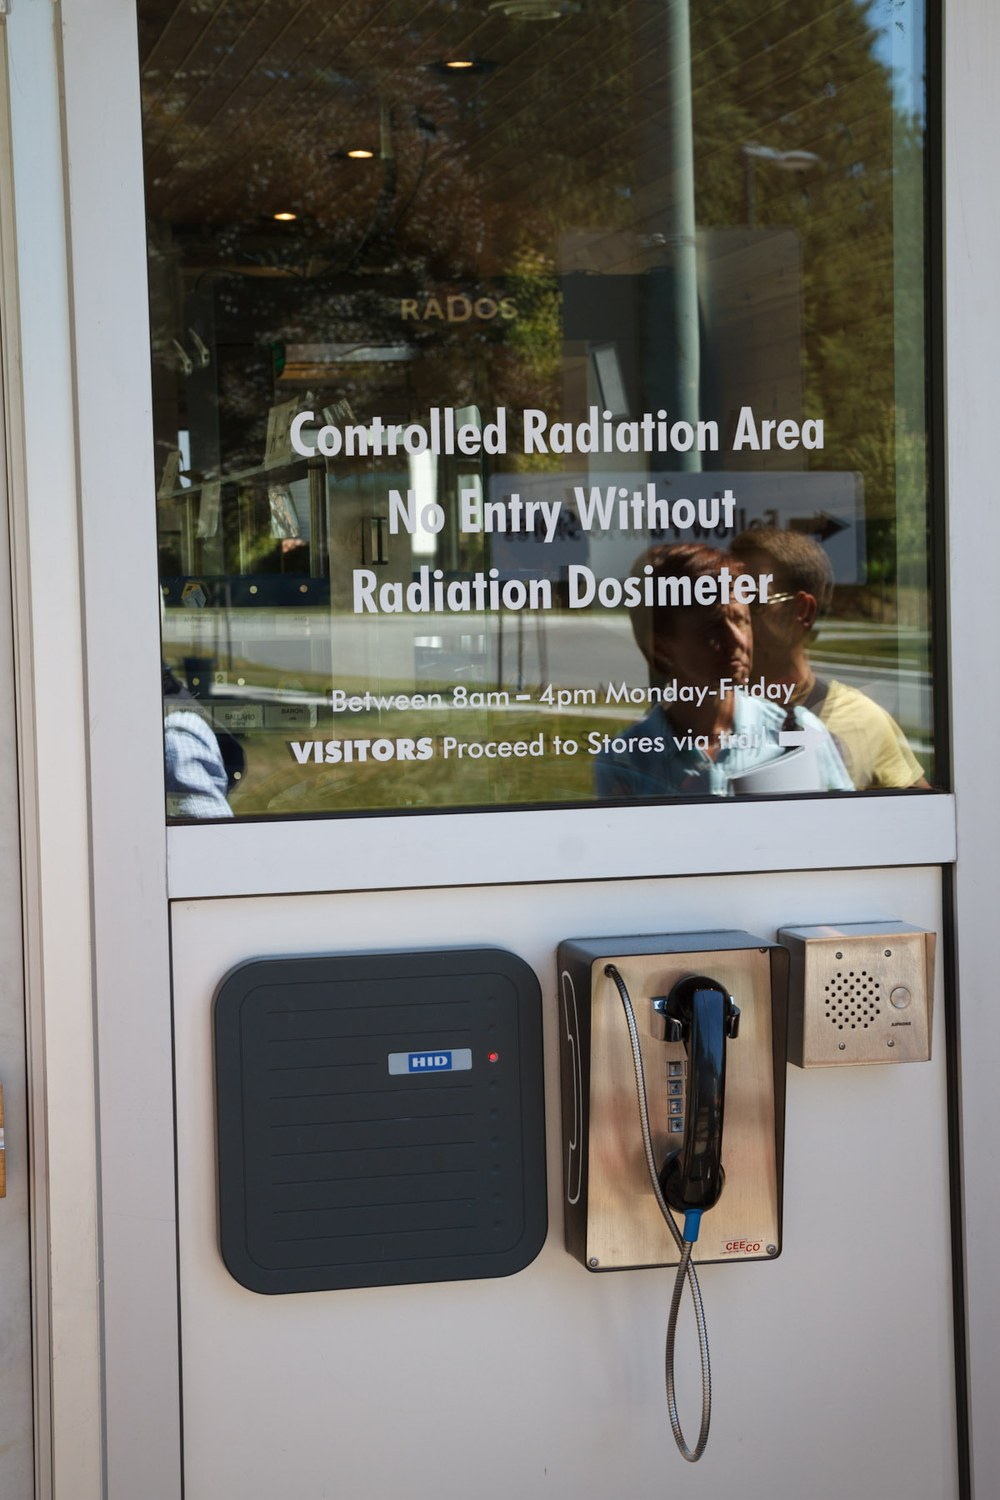
\includegraphics[width=0.60\textwidth]{../figures/triumf_cyclotron.jpg}
\caption{TRIUMF 回旋加速器：回旋运动的工程尺度。回旋加速器把回旋运动做成了机器：束流在磁场里一圈圈加速，而这正是本节『束流的三个刻度』里的回旋半径与周期；要把束流送到靶上，先得把相空间与发射度管住——这是加速器与等离子体束流共同的语言。}
\label{fig:photo-appax}
\figsource{Adam Foster，CC BY-SA 2.0（Wikimedia Commons）}
\end{figure}

\section{空间电荷与派文斯：等效电位差是束能的三十倍}
\label{sec:app-ax-spacecharge}

束流自己带电，所以它自己产生电场。轴向电流在束内产生的径向电场由
「电流密度除以电荷通量」给出：
\begin{equation}
E_r=\frac{j_b}{\varepsilon_0v_b}=\frac{565.884242}{8.8541878128\times10^{-12}\times3.095316\times10^{6}}
=2.064781\times10^{7}\ \mathrm{V\,m^{-1}},
\label{eq:app-ax-selfield}
\end{equation}
乘上束半径就是束内外的\textbf{等效电位差}：
\begin{equation}
\Delta V=E_rr_b=3.097171\times10^{6}\ \mathrm{V}=3.0972\ \mathrm{MV},
\qquad
\frac{\Delta V}{E_b/e}=30.971710.
\label{eq:app-ax-dv}
\end{equation}
这个数字值得停下来看一眼：束流自己产生的电位差是它自身能量的 $30.971710$ 倍。
换句话说，一束没有中和的 $40\ \mathrm{A}$、$100\ \mathrm{keV}$ 氘束，
其空间电荷势能远超束的动能——它会在几厘米内把自己撑开。
用 KV 包络方程（式~\eqref{eq:app-ax-kv}）的量级估计，未中和时
$10\ \mathrm{m}$ 内包络要膨胀 $8.024125\times10^{3}\ \mathrm{m}$，即 $8.0241\ \mathrm{km}$：
不是「稍微散一点」，而是根本传不出去。要让 $10\ \mathrm{m}$ 内只涨
$0.01\ \mathrm{m}$，广义派文斯必须压到 $1.447203\times10^{-6}$ 以下，
对应中和度 $f_n\ge0.9999988$（$99.99988\%$）。这个结论听上去荒谬，
但它正是中性束存在的理由：\textbf{把离子变成中性原子，空间电荷问题就整个消失}。

空间电荷有多强，用一个无量纲数就能说清——\textbf{派文斯}（perveance）：
\begin{equation}
\begin{aligned}
K&=\frac{I_b}{V^{3/2}}=1.264911\times10^{-6}\ \mathrm{A\,V^{-1.5}},\\
K_\mathrm{gen}&=\frac{2I_b}{I_A\beta^3\gamma^3}=1.161253,\\
I_A&=\frac{4\pi\varepsilon_0m_Dc^3}{e}=6.258076\times10^{7}\ \mathrm{A}=62.581\ \mathrm{MA}.
\end{aligned}
\label{eq:app-ax-perv}
\end{equation}
$K_\mathrm{gen}\sim1$ 意味着空间电荷势能与动能同量级——这又一次说明
$40\ \mathrm{A}$、$100\ \mathrm{keV}$ 的束流已经站在「空间电荷主导」的区域里。

引出端还有一条硬上限：Child--Langmuir 定律给出空间电荷限制电流密度
\begin{equation}
j_\mathrm{CL}=\frac{4\varepsilon_0}{9}\sqrt{\frac{2e}{m_D}}\frac{V^{3/2}}{d^2}
=3045.167317\ \mathrm{A\,m^{-2}}\quad(d=0.02\ \mathrm{m}),
\label{eq:app-ax-cl}
\end{equation}
在 $\pi r_b^2$ 的引出面上对应 $215.250194\ \mathrm{A}$，是需求 $40\ \mathrm{A}$ 的
$5.3813$ 倍；反过来，要引出 $40\ \mathrm{A}$ 只需要
$1.313557\times10^{-2}\ \mathrm{m^2}=131.3557\ \mathrm{cm^2}$ 的面积，
即半径 $0.064662\ \mathrm{m}=6.4662\ \mathrm{cm}$ 的一个圆。
余量 $5.3813$ 倍看着宽裕，但它是用 $0.02\ \mathrm{m}$ 的间隙换来的：
间隙越小，$j_\mathrm{CL}$ 越高，打火风险也越大——引出系统的设计就是在这两者之间找平衡。

\begin{table}[htbp]
\centering
\small
\caption{空间电荷的量级（声明：$I_b=40\ \mathrm{A}$、$E_b=100\ \mathrm{keV}$、$r_b=0.15\ \mathrm{m}$、$d=0.02\ \mathrm{m}$）}
\label{tab:app-ax-spacecharge}
\begin{tabular}{p{5.0cm}p{4.6cm}p{3.8cm}}
\hline
量 & 值 & 说明 \\
\hline
自场 $E_r$ & $2.064781\times10^{7}\ \mathrm{V\,m^{-1}}$ & $j_b/(\varepsilon_0v_b)$ \\
等效电位差 $\Delta V$ & $3.0972\ \mathrm{MV}$ & $E_rr_b$ \\
$\Delta V/(E_b/e)$ & $30.971710$ & 势能远超动能 \\
广义派文斯 $K_\mathrm{gen}$ & $1.161253$ & 空间电荷主导 \\
未中和膨胀（$10\ \mathrm{m}$） & $8.0241\ \mathrm{km}$ & 不可用 \\
所需中和度 & $99.99988\%$ & 所以要中性束 \\
Child--Langmuir 极限 & $3045.167317\ \mathrm{A\,m^{-2}}$ & 引出硬上限 \\
引出余量 & $5.3813$ 倍 & 需求 $40\ \mathrm{A}$ \\
\hline
\end{tabular}
\end{table}

\begin{tip}{空间电荷不是修正项，它是束流的主项}{tip-app-ax-spacecharge}
算束流时最容易被跳过的就是空间电荷：很多人先算发射度、算透镜，最后才「顺便」
看一眼空间电荷。但 $\Delta V/(E_b/e)=30.971710$ 说明顺序应该反过来——
先问「中和了没有」，再谈发射度。凡是电流到几十安培、能量到百 keV 量级的束流，
空间电荷都是主项，不是修正。
\end{tip}

{\footnotesize
\textbf{出处：}派文斯、广义派文斯、Child--Langmuir 定律与 KV 包络方程
参照 Humphries 与 Reiser 的教材；等效电位差与中和度要求的写法是本书自己的推导，
不复制原书的引出电极设计与程序。
}

\section{中和与残余离子：束流功率账}
\label{sec:app-ax-neutral}

中性束的「中性」是换来的：先引出离子束，再让它穿过气体靶做电荷交换，
一部分离子变成中性原子，剩下的仍是离子。声明中和效率 $\eta_\mathrm{neut}=0.55$、
气体靶线密度 $n_{gl}=10^{20}\ \mathrm{m^{-2}}$、剥离截面 $10^{-20}\ \mathrm{m^2}$：
\begin{equation}
\begin{aligned}
P_b&=I_bE_b/e=4.0000\ \mathrm{MW},\\
P_\mathrm{neut}&=\eta_\mathrm{neut}P_b=2.2000\ \mathrm{MW},\\
P_\mathrm{ion}&=(1-\eta_\mathrm{neut})P_b=1.8000\ \mathrm{MW}.
\end{aligned}
\label{eq:app-ax-power}
\end{equation}
气体靶的透过率按指数衰减：
\begin{equation}
T_\mathrm{cell}=e^{-n_{gl}\sigma L}=0.367879,
\label{eq:app-ax-trans}
\end{equation}
它和「中和效率」不是一回事：透过率说的是「有多少束流没有发生碰撞」，
中和效率说的是「碰撞之后有多少变成了中性原子」。设计气体靶时要同时看这两个数，
靶太薄则中和不足，靶太厚则中性原子又被剥掉。

中性原子进入等离子体后不再受磁场约束，靠电离被「抓住」。有效电离截面
$\sigma_\mathrm{eff}=10^{-20}\ \mathrm{m^2}$（与附录 M 同口径）给出射程
\begin{equation}
\lambda=\frac{1}{n_e\sigma_\mathrm{eff}}=1.000000\ \mathrm{m},
\qquad
\text{穿透份额}=e^{-R/\lambda}=2.029431\times10^{-3}=0.202943\%.
\label{eq:app-ax-range}
\end{equation}
$0.202943\%$ 就是从等离子体另一侧直接穿过去的部分，必须由第一壁承受。
剩下 $99.7971\%$（被吸收份额）被等离子体吸收，对应功率
$P_\mathrm{abs}=2.195535\ \mathrm{MW}$，摊在 $V=832.2\ \mathrm{m^3}$ 上
平均功率密度只有 $2638.2303\ \mathrm{W\,m^{-3}}$——这解释了为什么中性束
不会像激光那样把等离子体「打个洞」：它的能量是沿 $1\ \mathrm{m}$ 的射程
慢慢沉积的，而不是在 $1\ \mathrm{mm}$ 内集中释放。

\begin{table}[htbp]
\centering
\small
\caption{中性束的功率账（声明：$\eta_\mathrm{neut}=0.55$、$\sigma_\mathrm{eff}=10^{-20}\ \mathrm{m^2}$、$R=6.2\ \mathrm{m}$、$V=832.2\ \mathrm{m^3}$）}
\label{tab:app-ax-neutral}
\begin{tabular}{p{5.0cm}p{4.4cm}p{4.0cm}}
\hline
量 & 值 & 去向 \\
\hline
束功率 $P_b$ & $4.0000\ \mathrm{MW}$ & 引出 \\
中性份额 $P_\mathrm{neut}$ & $2.2000\ \mathrm{MW}$ & 进入等离子体 \\
残余离子 $P_\mathrm{ion}$ & $1.8000\ \mathrm{MW}$ & 偏转板带走 \\
靶透过率 & $0.367879$ & $e^{-n_{gl}\sigma L}$ \\
射程 $\lambda$ & $1.000000\ \mathrm{m}$ & $1/(n_e\sigma_\mathrm{eff})$ \\
穿透份额 & $0.202943\%$ & 打到第一壁 \\
吸收功率 & $2.1955\ \mathrm{MW}$ & 加热等离子体 \\
平均功率密度 & $2638.2303\ \mathrm{W\,m^{-3}}$ & 沿射程沉积 \\
\hline
\end{tabular}
\end{table}

\begin{tip}{中性化的目的不是效率，是让束流活下来}{tip-app-ax-neutral}
中和效率 $0.55$ 意味着 $45\%$ 的束功率被浪费掉——听起来很低。
但如果不做中和，空间电荷会让整束在 $10\ \mathrm{m}$ 内膨胀 $8.0241\ \mathrm{km}$
（AX.4），送到等离子体的功率是零。所以中和器的价值不能用「效率」衡量，
它买的是「束流能到达等离子体」这件事本身。$1.8000\ \mathrm{MW}$ 的残余离子
还必须由偏转板带走，这部分热负荷是中性束系统的主要工程约束之一。
\end{tip}

{\footnotesize
\textbf{出处：}中和效率、气体靶与射程的量级口径参照 ITER 中性束的公开技术文件
与 Hemsworth 等的综述；$\sigma_\mathrm{eff}=10^{-20}\ \mathrm{m^2}$ 与附录 M
保持同一口径，本书只借量级，不复制其束线几何与真空系统设计。
}

\section{束流在等离子体里停在哪里：临界能量与慢化路程}
\label{sec:app-ax-slowing}

中性原子被电离成快离子之后，它要把能量交给等离子体才能算「加热」。
交出去的过程由两种碰撞竞争：与电子的碰撞（阻力正比于速度）和与离子的碰撞
（阻力正比于 $1/v^2$）：
\begin{equation}
\begin{aligned}
F_e&=K_\mathrm{eff}\,v, &\quad K_\mathrm{eff}&=5.096269\times10^{-27}\ \mathrm{kg\,s^{-1}},\\
F_i&=\frac{C_i}{v^2}, &\quad C_i&=\frac{4\pi n_eZ_\mathrm{eff}e^4\ln\Lambda}{(4\pi\varepsilon_0)^2m_i}
=5.478026\times10^{-7}.
\end{aligned}
\label{eq:app-ax-drag}
\end{equation}
两者相等的地方就是\textbf{临界能量}：
\begin{equation}
\begin{aligned}
v_c&=\left(\frac{C_i}{K_\mathrm{eff}}\right)^{1/3}=4.754709\times10^{6}\ \mathrm{m\,s^{-1}},\\
E_c&=\frac{1}{2}m_Dv_c^2=3.780492\times10^{-14}\ \mathrm{J}=235.9598\ \mathrm{keV}=25.6645\,T_e.
\end{aligned}
\label{eq:app-ax-ec}
\end{equation}
换算成常用的定标 $14.8\,A\,T_e$（$A=2$，$T_e=9.194\ \mathrm{keV}$）得到
$272.1424\ \mathrm{keV}$，与上式相差 $1.1533$ 倍——两者同量级，
差别来自 $Z_\mathrm{eff}$、$m_i$ 与库仑对数口径；做设计时用精确式，
做量级判断时用定标式。

束能 $E_b=100\ \mathrm{keV}$ 只有 $E_c$ 的 $0.423801$ 倍，所以阻力以离子为主：
离子阻力是电子阻力的 $3.624574$ 倍，能量给离子的份额 $78.3764\%$。
「$100\ \mathrm{keV}$ 的束主要加热离子」这句话的定量版本就是这个数。
慢化时间由电子阻力定：
\begin{equation}
\tau_v=\frac{m_D}{K_\mathrm{eff}}=0.656263\ \mathrm{s},
\qquad
\tau_E=\frac{\tau_v}{2}=0.328132\ \mathrm{s},
\label{eq:app-ax-tau}
\end{equation}
但慢化时间不是「束流停下来的时间」——快离子一直在环里绕圈。
它与背景离子的速度比 $x=v_b/v_{Te}=0.054429$，落在阻力公式的线性段
（$G(x)$ 精确值与渐近值之比 $0.998224$，用哪个都行）。
慢化路程 $v_b\tau_v=2.031342\times10^{6}\ \mathrm{m}=2031.34\ \mathrm{km}$，
相当于绕环向周长 $2\pi R=38.955749\ \mathrm{m}$ 走 $52144.87$ 圈。

把两个长度并排看，本附录最重要的一句对比就出来了：中性束的射程是
$1.000000\ \mathrm{m}$（原子过程决定的），快离子的慢化路程是
$2031.34\ \mathrm{km}$（库仑碰撞决定的），两者相差 $2.031\times10^{6}$ 倍。
\textbf{「中性束打在哪里」由射程决定，「加热谁」由临界能量决定，
「能量怎么分配」由慢化过程决定}——三件事，三个不同的公式。

\begin{table}[htbp]
\centering
\small
\caption{慢化与临界能量（声明：$n_e=10^{20}\ \mathrm{m^{-3}}$、$T_e=9.194\ \mathrm{keV}$、$\ln\Lambda=17$、$Z_\mathrm{eff}=2$、$m_i=2.5\ \mathrm{u}$）}
\label{tab:app-ax-slowing}
\begin{tabular}{p{5.0cm}p{4.4cm}p{4.0cm}}
\hline
量 & 值 & 说明 \\
\hline
速度比 $x=v_b/v_{Te}$ & $0.054429$ & 线性段 \\
慢化时间 $\tau_v$ & $0.656263\ \mathrm{s}$ & $m_D/K_\mathrm{eff}$ \\
能量损失时间 $\tau_E$ & $0.328132\ \mathrm{s}$ & $\tau_v/2$ \\
临界能量 $E_c$ & $235.9598\ \mathrm{keV}$ & $25.6645\,T_e$ \\
定标 $14.8\,A\,T_e$ & $272.1424\ \mathrm{keV}$ & 相差 $1.1533$ 倍 \\
离子阻力/电子阻力 & $3.624574$ & 离子加热为主 \\
给离子的份额 & $78.3764\%$ & $E_b<E_c$ \\
慢化路程 & $2031.34\ \mathrm{km}$ & 绕环 $52144.87$ 圈 \\
中性束射程 & $1.000000\ \mathrm{m}$ & 相差 $2.031\times10^{6}$ 倍 \\
\hline
\end{tabular}
\end{table}

\begin{tip}{「打到哪」和「加热谁」是两件事}{tip-app-ax-slowing}
射程 $1.000000\ \mathrm{m}$ 说的是中性束在哪里被电离；临界能量
$235.9598\ \mathrm{keV}$ 说的是快离子把能量交给电子还是离子。
一束 $100\ \mathrm{keV}$ 的束（$E_b/E_c=0.423801$）主要加热离子，
而 $300\ \mathrm{keV}$ 的束就会把 $58.9084\%$ 的能量交给电子（练习 5）。
设计加热方案时，先定「想加热谁」，再选束能，最后用射程定注入几何——
顺序反了会得到「能量送到位了、但加热错了对象」的结果。
\end{tip}

\textbf{出处：}电子阻力与离子阻力的分段形式、临界能量与慢化时间参照
Stacey 与 Wesson 的教材（附录 W 已用同一组公式处理 $3.5\ \mathrm{MeV}$ 的
$\alpha$ 粒子）；本书只借公式结构，不复制其快离子分布演化与输运结果。
\begin{figure}[htbp]
\centering
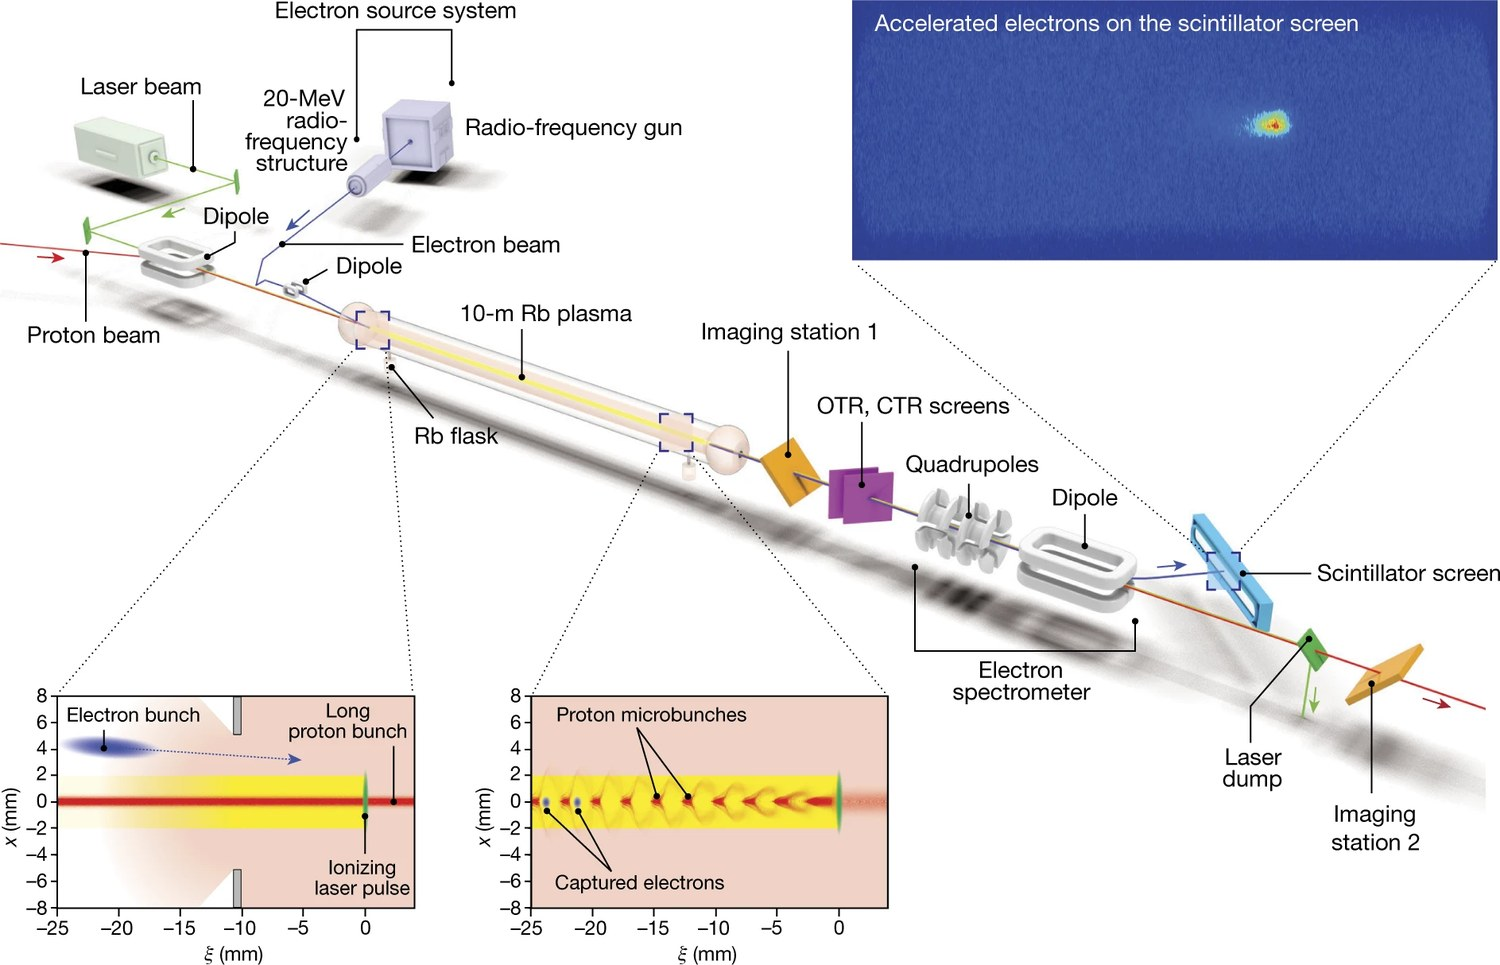
\includegraphics[width=0.72\textwidth]{../figures/ax_awake_wakefield.jpg}
\caption{等离子体不只被加速器诊断，它本身就能当加速器：质子束在等离子体里激起尾场，把电子在厘米尺度上加速到 GeV。本节讲束流与等离子体耦合，这是最直接的证据。}
\label{fig:photo-appax2}
\figsource{E. Adli 等（AWAKE 合作组，Nature 561, 363），CC BY 4.0（Wikimedia Commons）}
\end{figure}

\section{束流与等离子体耦合：冷束双流模与稳定化门槛}
\label{sec:app-ax-coupling}

前面几节把束流当成「在真空里飞的电荷云」。一旦它进了等离子体，就多了一个自由度：
束流可以把自己的动能交给等离子体波。最经典的通道是\textbf{双流不稳定性}
（two-stream instability）：束内等离子体频率
\begin{equation}
\begin{aligned}
\omega_{pb}&=\sqrt{\frac{n_be^2}{\varepsilon_0m_D}}=3.145045\times10^{7}\ \mathrm{rad\,s^{-1}}
\quad(f_{pb}=5.005495\ \mathrm{MHz}),\\
\omega_{pe}&=\sqrt{\frac{n_ee^2}{\varepsilon_0m_e}}=5.641460\times10^{11}\ \mathrm{rad\,s^{-1}},
\end{aligned}
\label{eq:app-ax-wp}
\end{equation}
「冷束」极限下的最大增长率是
\begin{equation}
\gamma_\mathrm{ts}=\frac{\sqrt{3}}{2}\left(\frac{n_b}{2n_e}\right)^{1/3}\omega_{pe}
=8.730040\times10^{9}\ \mathrm{rad\,s^{-1}},
\qquad
\frac{1}{\gamma_\mathrm{ts}}=1.145470\times10^{-10}\ \mathrm{s}=0.1145\ \mathrm{ns}.
\label{eq:app-ax-ts}
\end{equation}
$0.1145\ \mathrm{ns}$ 比慢化时间 $0.656263\ \mathrm{s}$（AX.6）快十个数量级。
如果这条通道真的畅通，束流会在进入等离子体的瞬间就「热化」掉，
中性束根本不可能把能量送到芯部。它为什么没有发生？答案在共振波数上：
束流与等离子体波共振的波数是 $k=\omega_{pe}/v_b=1.822580\times10^{5}\ \mathrm{m^{-1}}$，
对应的 $k\lambda_{De}=12.991461$，电子 Landau 阻尼率只有
$\gamma_L/\omega_{pe}=6.358104\times10^{-5}$——阻尼很弱，所以问题不在电子。

真正起作用的是束流自己的速度展宽。源的发散角 $\theta_{bl}=0.30^\circ$ 意味着
束流在速度空间里有 $\Delta v/v_b\sim\theta_{bl}$ 的展宽，它把共振条件抹开：
\begin{equation}
k\Delta v=\omega_{pe}\theta_{bl}=2.953862\times10^{9}\ \mathrm{rad\,s^{-1}},
\qquad
\frac{\gamma_\mathrm{ts}}{k\Delta v}=2.955467.
\label{eq:app-ax-kdv}
\end{equation}
两个数只差 $2.955467$ 倍——这就是真实情况：冷束极限给出的增长被展宽削掉大半，
剩下一个「同一量级」的竞争。束流不会瞬间热化，但也不会完全安稳；
到底长不长起来，取决于速度分布尾部与实际磁场几何——那已经属于附录 W
的快离子模与附录 AE 的动理学范畴，本附录只把门槛摆在桌面上。

顺带记住穿越时间：束流以 $v_b$ 穿过 $R=6.2\ \mathrm{m}$ 只需要
$2.003027\times10^{-6}\ \mathrm{s}=2.0030\ \mathrm{\mu s}$，
在冷束极限下相当于 $17486.5$ 个 e 折。做束流实验时，微秒量级的时间分辨
不是「高配」，而是必需品。

\begin{table}[htbp]
\centering
\small
\caption{束-等离子体耦合的两个频率与一个门槛（声明：$n_b=1.141070\times10^{15}\ \mathrm{m^{-3}}$、$n_e=10^{20}\ \mathrm{m^{-3}}$、$v_b=3.095316\times10^{6}\ \mathrm{m\,s^{-1}}$）}
\label{tab:app-ax-coupling}
\begin{tabular}{p{5.0cm}p{4.4cm}p{4.0cm}}
\hline
量 & 值 & 说明 \\
\hline
束内频率 $f_{pb}$ & $5.005495\ \mathrm{MHz}$ & 与 $n_b$ 有关 \\
等离子体频率 $\omega_{pe}$ & $5.641460\times10^{11}\ \mathrm{rad\,s^{-1}}$ & 与 $n_e$ 有关 \\
冷束增长率 $\gamma_\mathrm{ts}$ & $8.730040\times10^{9}\ \mathrm{rad\,s^{-1}}$ & 上限 \\
冷束增长时间 & $0.1145\ \mathrm{ns}$ & 比慢化快十个量级 \\
共振 $k\lambda_{De}$ & $12.991461$ & 电子阻尼弱 \\
Landau 阻尼率 & $6.358104\times10^{-5}$ & $\gamma_L/\omega_{pe}$ \\
展宽门槛 $k\Delta v$ & $2.953862\times10^{9}\ \mathrm{rad\,s^{-1}}$ & 源发散角决定 \\
$\gamma_\mathrm{ts}/(k\Delta v)$ & $2.955467$ & 同一量级竞争 \\
穿越时间 & $2.0030\ \mathrm{\mu s}$ & 合 $17486.5$ 个 e 折 \\
\hline
\end{tabular}
\end{table}

\begin{tip}{「冷束」既是优点，也是风险}{tip-app-ax-coupling}
冷束（$T_\mathrm{eff}=2.741557\ \mathrm{eV}$）意味着相空间面积小、可聚焦，
但冷也意味着速度展宽小，共振条件抹不开，不稳定性容易长起来。
$\gamma_\mathrm{ts}/(k\Delta v)=2.955467$ 说明在这个工作点上两者刚好同量级：
想把束流做得更冷（提高亮度），就要同时准备好抑制不稳定性的手段，
比如让能量分布稍宽一点、或者把束流切成更短的时间片（$2.0030\ \mathrm{\mu s}$ 的穿越时间
就是「短」的标尺）。
\end{tip}

{\footnotesize
\textbf{出处：}冷束双流不稳定性的增长率、共振条件与 Landau 阻尼口径参照
Krall 与 Trivelpiece 的等离子体物理教材以及附录 AE 的动理学口径；
本书只借公式形式与量级，不复制其色散关系的完整推导与数值解。
}

\section{估算练习}
\label{sec:app-ax-problems}

\textbf{练习 1} 一束 $80\ \mathrm{keV}$ 的氘束，求速度、$\beta$ 与在 $5.3\ \mathrm{T}$
磁场里的回旋半径。

\textbf{解答 1} $v=\sqrt{2E_b/m_D}=2.768534\times10^{6}\ \mathrm{m\,s^{-1}}$，
$\beta=0.009235$，$\rho_c=m_Dv/(eB)=0.010904\ \mathrm{m}=1.0904\ \mathrm{cm}$。
回旋半径与 $\sqrt{E}$ 成正比：能量降到 $80.0000\%$ 时，
回旋半径降到 $89.4427\%$（只降 $10.5573\%$）。

\textbf{练习 2} 若小孔半径改成 $4\ \mathrm{mm}$、发散角改成 $0.25^\circ$，
求发射度、归一化发射度与 $\beta^*=2.0\ \mathrm{m}$ 处的束腰。

\textbf{解答 2} $\varepsilon=4.0\times10^{-3}\times4.363323\times10^{-3}
=1.745329\times10^{-5}\ \mathrm{m\,rad}$（即 $0.0174533\ \mathrm{mm\,mrad}$），
$\varepsilon_n=\beta\gamma\varepsilon=1.802124\times10^{-7}\ \mathrm{m\,rad}$，
$\sigma_x=\sqrt{\varepsilon\beta^*}=5.9082\ \mathrm{mm}$。
小孔半径缩到 $80.0000\%$、发散角缩到 $83.3333\%$，发射度比 AX.2 降了 $33.3333\%$，
束腰从 $7.2360\ \mathrm{mm}$ 降到 $5.9082\ \mathrm{mm}$（降 $18.3503\%$）。

\textbf{练习 3} 一束 $25\ \mathrm{A}$ 的束，半径 $0.12\ \mathrm{m}$（其他条件同 AX.4），
求电流密度、自场与等效电位差相对于束能的倍数。

\textbf{解答 3} $j=25/(\pi\times0.12^2)=552.6213\ \mathrm{A\,m^{-2}}$，
$E_r=j/(\varepsilon_0v_b)=2.016387\times10^{7}\ \mathrm{V\,m^{-1}}$，
$\Delta V/(E_b/e)=E_rr_b/(E_b/e)=24.1966$。
电流降到 $62.5000\%$、半径降到 $80.0000\%$，倍数只从 $30.971710$ 降到 $24.1966$——
空间电荷对参数不敏感，这正说明它「躲不掉」。

\textbf{练习 4} 若引出电压升到 $120\ \mathrm{kV}$、间隙改成 $0.025\ \mathrm{m}$，
求 Child--Langmuir 极限电流密度与 $\pi r_b^2$ 上的极限电流。

\textbf{解答 4} $j_\mathrm{CL}=\frac{4\varepsilon_0}{9}\sqrt{2e/m_D}V^{3/2}/d^2
=2561.9049\ \mathrm{A\,m^{-2}}$，
$I_\mathrm{CL}=j_\mathrm{CL}\pi r_b^2=181.0904\ \mathrm{A}$。
电压升到 $120.0000\%$、间隙升到 $125.0000\%$，极限反而从 $215.250194\ \mathrm{A}$ 降到
$181.0904\ \mathrm{A}$（$84.1302\%$）——因为 $j_\mathrm{CL}\propto V^{3/2}/d^2$，间隙的平方更狠。

\textbf{练习 5} 一束 $300\ \mathrm{keV}$ 的氘束（其他条件同 AX.6），求速度、
$v/v_{Te}$、离子阻力与电子阻力之比，以及给电子的能量份额。

\textbf{解答 5} $v=5.361244\times10^{6}\ \mathrm{m\,s^{-1}}$，
$v/v_{Te}=0.094273$，$F_i/F_e=0.697550$，
给电子的份额 $58.9084\%$。与 $100\ \mathrm{keV}$ 的束（给离子 $78.3764\%$）
正好反过来：束能跨过 $E_c=235.9598\ \mathrm{keV}$ 之后，加热对象就换了。

\textbf{练习 6} 若中和效率只有 $0.45$，$40\ \mathrm{A}$、$100\ \mathrm{keV}$ 的束
有多少功率进入等离子体？多少功率要由偏转板带走？

\textbf{解答 6} $P_\mathrm{neut}=0.45\times4.0000\ \mathrm{MW}=1.8000\ \mathrm{MW}$，
$P_\mathrm{ion}=0.55\times4.0000\ \mathrm{MW}=2.2000\ \mathrm{MW}$。
注意与 AX.5 的 $\eta_\mathrm{neut}=0.55$ 相比：中和效率从 $0.55$ 降到 $0.45$，
进入等离子体的功率少 $0.4000\ \mathrm{MW}$（$18.1818\%$），而偏转板的热负荷
增加 $0.4000\ \mathrm{MW}$（$22.2222\%$）——两个方向都要付账。

\section{来源、分级与版权说明}
\label{sec:app-ax-source}

\begingroup\small
本附录的定义、判据与公式形式取自下列公开来源，按借鉴程度分级列出：

\begin{table}[htbp]
\centering
\small
\caption{本附录的借鉴来源}
\label{tab:app-ax-source}
\begin{tabular}{p{0.6cm}p{6.2cm}p{7.0cm}}
\hline
序号 & 来源 & 借用了什么 \\
\hline
1 & Humphries, \emph{Charged Particle Beams}（Wiley, 1990） & 发射度、亮度、派文斯与束包络的基本框架 \\
2 & Reiser, \emph{Theory and Design of Charged Particle Beams}（2nd ed., Wiley, 2008） & KV 包络方程；空间电荷主导判据与匹配概念 \\
3 & Wiedemann, \emph{Particle Accelerator Physics}（4th ed., Springer, 2015） & Twiss 参数、归一化发射度与亮度的定义 \\
4 & Speth 等，\emph{Nucl. Fusion} 46, S220 (2006) & 射频负离子源的束流发散角与单孔电流量级 \\
5 & Hemsworth 等，\emph{Nucl. Fusion} 49, 045006 (2009) & ITER 中性束的中和效率、残余离子与束线构成 \\
6 & Wesson, \emph{Tokamaks}（4th ed., Oxford, 2011） & 快离子慢化与临界能量的处理方式 \\
7 & Stacey, \emph{Fusion Plasma Physics}（2nd ed., Wiley, 2011） & 电子阻力与离子阻力的分段形式、慢化时间 \\
8 & Krall \& Trivelpiece, \emph{Principles of Plasma Physics}（McGraw-Hill, 1973） & 冷束双流不稳定性增长率与共振条件 \\
\hline
\end{tabular}
\end{table}

\textbf{不复制声明：}本附录只借用上述来源的定义、判据形式与量级口径；
不复制其束光学设计程序、电极与束线几何、相空间匹配方法、实验数据与习题。

\textbf{本附录不给什么：}不给完整的束光学设计（磁透镜布置、色差与球差校正）、
不给离子源的等离子体放电物理（那属于附录 AH 与 AO 的范畴）、
不给中性束注入对等离子体剖面演化的输运结果（那属于附录 M 与 W），
也不给束流诊断的具体硬件方案。需要做真实束线设计时，
应当使用经过验证的束光学程序，本附录的作用是把「该问哪几个问题、量级是多少」
讲清楚。

\textbf{分级：}AX.1--AX.6 属于「读过本章后能自己复算」的层级；
AX.7 的双流模门槛与 AX.5 的中和效率属于「知道结论、会用量级」的层级；
束光学匹配与快离子模的完整动理学属于进阶内容，正文只给判据。
\endgroup
